
\documentclass[journal]{IEEEtran}

\usepackage{amsmath}
\usepackage{xcolor}
\usepackage{graphicx}
\graphicspath{ {./images/} }
\usepackage[super]{nth}
\usepackage{tabularx,booktabs}
% defined centered version of "X" column type:
\newcolumntype{C}{>{\centering\arraybackslash}X} 
\setlength{\extrarowheight}{1pt} % for a bit more open "look"
\usepackage{lipsum} % filler text
\usepackage{caption}
\usepackage{algpseudocode}
\usepackage{algorithm}
\usepackage{amsmath}
\usepackage{multirow}
\usepackage{setspace}

\usepackage[section]{placeins}
% \raggedbottom



% correct bad hyphenation here
\hyphenation{optical networks semiconductor}


\begin{document}

% paper title
\title{Fanorona: Unbeatable AI player}

% AUTHORS
\author{Catia~Teixeira,~\IEEEmembership{Student,~FEUP,}
        Rojan~Aslani,~\IEEEmembership{Student,~FEUP}}% 


% The paper headers
\markboth{Master's in data science and engineering, Artificial Intelligence, February~2023}
{Shell \MakeLowercase{\textit{et al.}}: Bare Demo of IEEEtran.cls for IEEE Journals}
% The only time the second header will appear is for the odd-numbered pages

\maketitle

\begin{abstract}
Fanorona is a two-player board game that has been played for hundreds of years by Malagasy. This article provides an overview of the game rules and complexity analysis, as well as a detailed description of the methodology and implementation details of three different artificial intelligence (AI) algorithms that play Fanorona. The authors aimed to evaluate the algorithms' performance in different game scenarios, including games played between human players, between human and computer players, and between two computer players. Moreover, three board sizes and three difficulty levels are available for configuration. The implemented AI algorithms are Minimax, Minimax with Alpha-Beta Pruning, and Monte Carlo Tree Search (MCTS). The results showed that MCTS on average is slower in making a move in comparison to the Minimax algorithms. However, it has a higher chance of winning in smaller board sizes, with fewer moves. All three AI players were able to win against a random player. Moreover, it was interesting to observe that even though it tends to be slower, MCTS seems to be able to adopt a more offensive attitude in the game. It would be interesting to further explore the hyper-parameter tuning of the algorithms in future works.

\end{abstract}

\begin{IEEEkeywords}
Fanorona, Board game, Adversarial Search, Artificial Intelligence, Minimax, Monte Carlo Tree Search.
\end{IEEEkeywords}

\IEEEpeerreviewmaketitle

%% INTRODUCTION %%
\section{Introduction}
\IEEEPARstart{F}{anorona} is a two-player strategic board game that originated in Madagascar. Its rules are quite similar to those of the game of checkers, but it has its own unique features~\cite{gen2012}.

%\subsection{Specification of the work}

Fanorona is played with black and white stones placed on a rectangular board. The size of the board varies depending on the variant of the game being played. The three standard variants are Fanoron-Telo (3 by 3), Fanoron-Dimy (5 by 5), and Fanoron-Tsivy (5 by 9). An example of the Fanaron-Tsivy board is presented in Fig.~\ref{fig:9x5Fano} \cite{walker2014book}. 

Players alternate turns, starting with White. Each player has 22 stones of their color on the board. The stones are placed where the grid lines cross, leaving the central point empty. A line represents the path along which a stone can move during the game. There are crossings that are strong and weak. In weak intersections, only horizontal and vertical moves are possible, while in a strong intersection, it is also possible to move a stone diagonally \cite{walker2014book, Schadd2008}. 

There are two kinds of moves: non-capturing (\emph{paika} move) and capturing. A \emph{paika} move consists of moving one stone along a line to an adjacent intersection without removing any of the opponent's stones.
Capturing moves, which imply the removal of one or more stones of the opponent, are necessary for a win and have to be played in preference to \emph{paika} moves. There are two ways to do a capturing move: 

% Fig.~\ref{fig:9x5Fano}
\begin{figure}[h]
    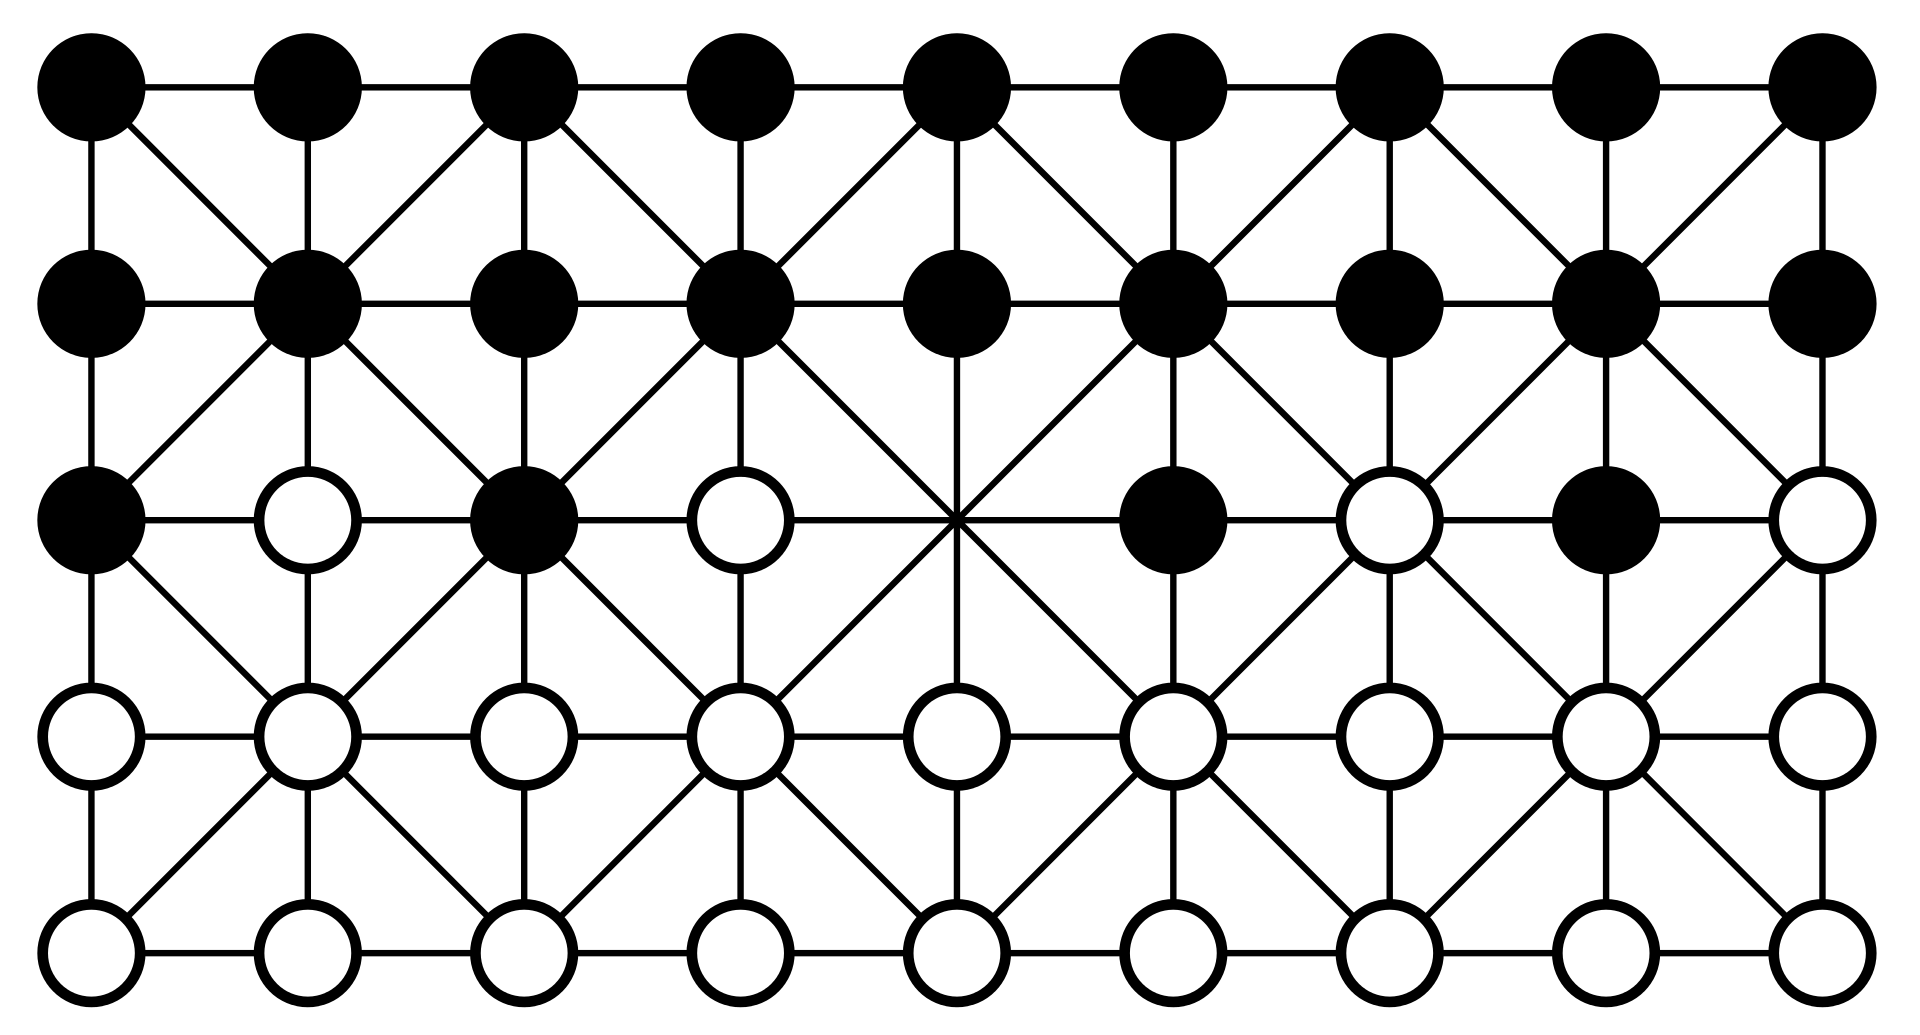
\includegraphics[width = 8cm]{Fanorona9x5}
    \centering
    \caption{Fanoron-Tsivy board (5x9) with the initial position of the stones \cite{Schadd2008}.}
    \label{fig:9x5Fano}
\end{figure}

\begin{enumerate}
    \item \textbf{Approach:} moving the capturing stone to a point adjacent to an opponent's stone, which must be on the continuation of the capturing stone's movement line.
    \item \textbf{Withdrawal:} the capturing stone moves from a point adjacent to the opponent's stone, away from the stone along the continuation of the line between them.
\end{enumerate}

When an opponent stone is captured, all opponent stones in line beyond that stone (as long as there is no interruption by an empty point or an own stone) are captured as well. Approach and withdrawal captures cannot be made at the same time – the player must choose one or the other.

The capturing stone is allowed to continue making successive captures, with the following restrictions:
\begin{itemize}
  \item The stone is not allowed to arrive at the same position twice.
  \item It is not permitted to move twice consecutively in the same direction (first to make a withdrawal capture, and then to make an approach capture) as part of a capturing sequence.
\end{itemize}

The winner is chosen when they take all the opponent's stones or leave the opponent in a position where they can't move. If neither player manages to win, then the game is a draw \cite{walker2014book}. According to several authors, when reaching the perfect play level, the game tends to reach a draw condition \cite{Schadd2008}, \cite{draw2015}.


\subsection{Complexity analysis}
It is important to quantify the game's complexity as it allows analysis of the difficulty of the game and allows choosing the most adequate techniques. According to \cite{Schadd2008}, after performing 10,000 games by Alpha-Beta players, Fanoron-Tsivy was estimated to have a game-tree complexity of $10^{46}$. Moreover, the space complexity was calculated to be $10^{21}$. These values are comparable to those of the game of checkers, which has a game-tree complexity and state-space complexity of $10^{31}$ and $10^{20}$, respectively \cite{Schaeffer2007}. However, the game-tree and state-space complexity of Fanorona is somewhat higher than those of checkers.


\subsection{Related work}

It is interesting to mention that up till now, Fanorona has never been strongly solved.
A different number of strategies and techniques have been developed in the past towards solving the game. According to \cite{draw2015}:

\subsubsection{The Minimax algorithm} The basic and classic approach technique is used for a variety of two-player games. The most popular variant is the Alpha-Beta pruning.
\subsubsection{The WINIMAX algorithm} This algorithm tries to maximize the win probability based on Minimax and the computing of $p_{win}$.
\subsubsection{The Memory Test (MT) framework} Based on null-window searches and transposition tables, this is a high-level game-tree search resulting in a best-first behavior of depth-first, classic Alpha-Beta search algorithm.
\subsubsection{The Monte Carlo Tree Search (MCTS) algorithm} This algorithm is based on simulations of full-game and applying the sequence of actions that lead to a higher number of wins.
\subsubsection{The opening book} This is a general, well-known technique for solving board games. Some positions are stored at the start of the game with the best moves for each of them. These openings may be proposed by human experts on the specific game.
\subsubsection{The proof number search algorithm} A general algorithm that is able to determine if a given goal can be achieved. A best-first algorithm that requires all nodes to be stored in memory.
\subsubsection{The rote learning} Memorizes encountered results, saving time for later occurrences by retrieving the stored results and increasing perfect-play performance. Gaining experience over time, its performance improves.
\subsubsection{The endgame databases} This technique consists of computed tables that contain the optimal solutions for a specific endgame or a set of endgames in a game. They provide a complete and optimal solution to a specific sub-problem of the game. One big part in its implementation is the optimization of retrieval and storage.


%% METHODOLOGY %%
% Section~\ref{section:Methodology}.
\section{Methodology}
\label{section:Methodology}

As this project focuses on two players with conflicting goals who are trying to explore the same search space for the solution, this project is formulated as an adversarial search problem. Fanorona's environment is accessible, deterministic, non-episodic, static, and discrete, hence, it is a reasonable game to solve by computer. In this section, we will discuss the details of the formulation and implementation of the project. 


\subsection{Formulation of the problem}
The source code for the Fanorona board and the Minimax agent was obtained from \emph{marcogx}'s GitHub repository\footnote{https://github.com/marcogx/Fanorona-Game-AI}, and the source code for MCTS player was obtained from \emph{ahenrij}'s Github repository \footnote{https://github.com/ahenrij/fanorona}.
Withal vast alterations were applied to the code to adapt to several configurations, adding new AI players, organizing the code in different classes, as well as adding and adjusting several base functionalities.

The initial state of the game is demonstrated in Fig.~\ref{fig:9x5Fano}.
The operators for the movements of the stones were defined according to the position of the stone, more specifically, in each of the intersections, the possible directions of the movement were denoted. The variety of board sizes made it challenging to automatize this function at this point, however, in future works a more efficient way of doing these operations could be explored. 
The evaluation function is presented in Eq.~\ref{eq:player_points} and Eq.~\ref{eq:eval_func} and will be explained in detail in the upcoming subsections.
The objective test for this game is quite simple, aiming to remove all stones of the opponent on the board, and leaving none behind. Hence, the objective test is whether the number of opponent stones is equal to zero. 


\subsection{Implementation details}

To implement the Fanorona board game, Python programming language was used in Visual Studio Code and PyCharm Community integrated development environments. In total six modules were created:

\begin{enumerate}
    \item \textbf{main.py:} main control log
    \item \textbf{player.py:} generates and controls the different types of players
    \item \textbf{game.py:} controls general functionalities, including making moves and user interface (UI) control
    \item \textbf{board.py:} represents the game board
    \item \textbf{stats.py:} generates records about the configuration of the game, the time duration, the number of moves, and the winner, and exports them into a Comma Separated Values (CSV) file in a  tabular format
    \item \textbf{config.py:} holds global variables that are used and have to be uniform within all files
    
\end{enumerate}

A Graphical UI (GUI) was developed using pygame package. The GUI allows the user to configure the game by defining the following parameters:

\begin{itemize}
  \item Game mode: Computer-Computer, Human-Computer, Human-Human
  \item \nth{1} and \nth{2} players: Human, Minimax, Minimax with Alpha-Beta pruning, MCTS
  \item Board size: 3x3, 5x5, 9x5
  \item Difficulty: Easy, Medium, Hard
\end{itemize}

% approach
\subsection{Approach}

\subsubsection{Evaluation function (Heuristic)}
The proposed heuristic function was used both as the evaluation function for Minimax agents and as a biasing function for MCTS agent. The function basically compares the chance of winning of each of the players at a given game state, according to the number of stones present on the board, as well as the position of the stones (extra points for strong intersections), as indicated in Eq.~\ref{eq:player_points}. The overall score is calculated by subtracting the opponent's points from the player's point, and dividing it by the total point, as demonstrated in Eq.~\ref{eq:eval_func}.

% Eq.~\ref{eq:player_points}
\begin{multline}
    \label{eq:player_points}
    points = Number~of~player's~stones \\
     + 0.5 \times stones~on~strong~intersections
\end{multline}

% Eq.~\ref{eq:eval_func}
\begin{equation}
    \label{eq:eval_func}
    \frac {Player~points - Opponent~points}{Player~points + Opponent~points}
\end{equation}

\subsubsection{Draw condition}
In this program, the game is considered a draw when the players repeat three consecutive moves.

\subsubsection{Hint button}
For the human-computer game mode, a hint button was implemented. The button is only available in this mode and the optimal move is shown only after clicking on the hint button. This functionality uses a Minimax with Alpha-Beta pruning Agent with a maximum search depth of 2.

% D. Implemented algorithms
\subsection{Implemented algorithms}
Several computer agents were implemented, as mentioned earlier. The simplest one is the Random agent, followed by AI agents such as Minimax, Minimax with Alpha-Beta pruning, and MCTS. The AI agents are all utility-based agents and act based not only on what the goal is but also on the best way to reach that goal.

\subsubsection{\textbf{Random Agent}}
The random agent was used as the computer player in easy mode. As the name implies, this agent makes random moves by getting the list of all possible moves and choosing the first one in the list.

\subsubsection{\textbf{Minimax Agent}}
The Minimax algorithm is a basic depth-first search algorithm. It is an approach to create an AI engine for any Zero-Sum, perfect Information, two players games. The two players are identified as MIN and MAX.  It is a recursive algorithm that proceeds all the way down to the leaves of the tree and then backs up through the tree as the recursion unwinds \cite{russell2020}.  The most popular variant of the Minimax algorithm is the Alpha-Beta pruning \cite{Knuth1975}. 

The optimal strategy of this algorithm is determined by working out the Minimax value of each state of the tree. This value is the utility of being in that state, assuming both players play optimally until the end of the game. MAX prefers to move to a state of maximum value when it is its turn to move, while MIN prefers a state of minimum value (see Fig.~\ref{fig:minimax}) \cite{russell2020}.

Once the algorithm reaches the maximum depth, it uses the evaluation function (Eq.~\ref{eq:eval_func}) to choose the higher-scoring move. The pseudo-code for the implementation of Minimax algorithm in this Fanorona game can be found in Appendix~\ref{codeM}.

% Fig.~\ref{fig:minimax}
\begin{figure}[h!]
    \centering
    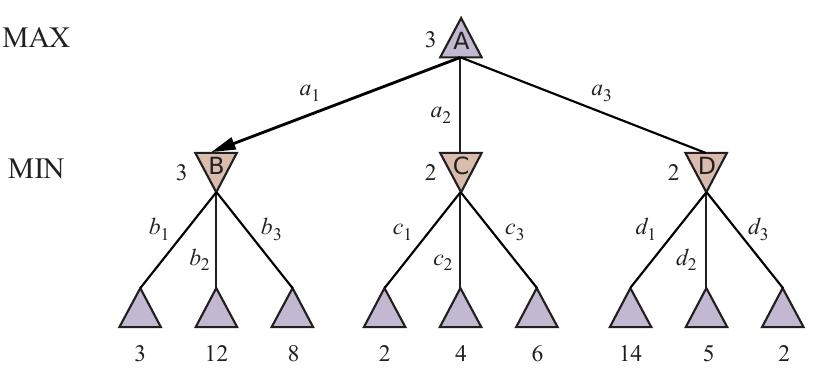
\includegraphics[width = 8cm]{minimax}
    \caption{Outline of Minimax \cite{russell2020}.}
    \label{fig:minimax}
\end{figure}

In this work, the difficulty of the game was defined by the depth of the Minimax algorithm, as demonstrated in Tab.~\ref{tab:Minimax_details}. The depth of the search tree is decreased for Fanoron-Tsivy boards. This adjustment was done to avoid prolonged decision-making time of the agents, due to the big size of the search space.
With the decrease of the depth by just 1 value, the agent became much faster, and the game was playable in reasonable time intervals.

\subsubsection{\textbf{Minimax with Alpha-Beta pruning}}
When using Minimax algorithm, the number of game states grows exponentially as the depth of the tree increases. This can become problematic in terms of computational capacity.

The benefit of alpha–beta pruning lies in the fact that branches of the search tree can be eliminated.
Given a position, if the player has a better choice either at the same level of the tree or at any point higher up in the tree, it will choose not to explore that branch further and not to move to that position \cite{russell2020}. To implement Minimax with Alpha-Beta pruning, two additional parameters are added to the Minimax algorithm, describing the bounds on the backed-up values that appear in the path:

\begin{itemize}
  \item Alpha ($\alpha$): value of highest valued choice found so far
  \item Beta ($\beta$): value of lowest valued choice found so far
\end{itemize}

These values are updated as the algorithm goes through the tree and prunes the remaining branches at a node as soon as the value is known to be worse than the current value for $\alpha$ or $\beta$ for MAX or MIN, respectively (see Fig.~\ref{fig:alphabeta}) \cite{russell2020}. The pseudo-code of this AI algorithm can be found in Appendix~\ref{Appendix:codeAB}.
The depths for each difficulty level of the game are demonstrated in Tab.~\ref{tab:Minimax_details}. 

A problem worth mentioning once limiting the search depth on both Minimax and Minimax with Alpha-Beta pruning is the horizon effect. When searching with depth limits, the algorithm can possibly make a move that results in a loss, without being able to detect the consequences in the current depth of the tree. Similarly, the optimal moves may be beyond the reach of the maximum tree depth. This can lead these algorithms to be at a disadvantage and can lead to the agents reaching loops in the game.

% Fig.~\ref{fig:alphabeta}
\begin{figure}[h!]
    \centering
    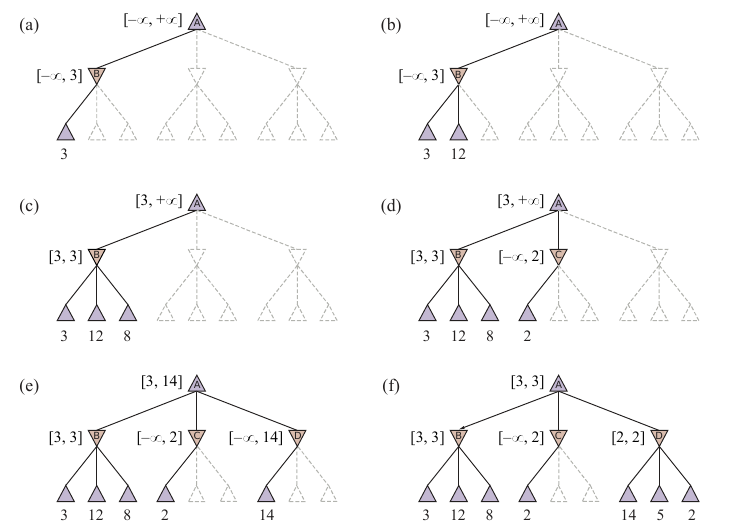
\includegraphics[width = 8cm]{alphabeta}
    \caption{Outline of Minimax with Alpha-Beta pruning (stages in alphabetical  order.) \cite{russell2020}}
    \label{fig:alphabeta}
\end{figure}

% Tab.~\ref{tab:Minimax_details}
\begin{table}[h]
    \caption{Parameter setting of different difficulty levels and board sizes for Minimax and Minimax with Alpha-Beta pruning algorithms (d: Maximum depth).}
    \centering
    \label{tab:Minimax_details}
        \begin{tabular}{l c c c c c}
        \hline
        Difficulty & Board size & Minimax d & Minimax-$\alpha\beta$ d\\
        \hline
        Medium & 3x3 & 3 & 3\\
        Medium & 5x5 & 3 & 3\\
        Medium & 9x5 & 2 & 2\\
        \addlinespace
        Hard & 3x3 & 4 & 5\\
        Hard & 5x5 & 4 & 5\\
        Hard & 9x5 & 3 & 4\\
        \hline
        \end{tabular}
\end{table}

\subsubsection{\textbf{Monte Carlo Tree Search (MCTS)}}

The basic MCTS strategy does not use a heuristic evaluation function, using instead an estimation of the state by averaging the utility over several simulations of complete games from the given state. As shown in Fig.~\ref{fig:Outline_MCTS}, the algorithm goes through 4 steps repeatedly:

\begin{enumerate}
    \item \textbf{Selection}: choose a move - starting from the root of the search tree, guided by the selection policy
    \item \textbf{Expansion}: grow the search tree by generating a new child for the selected node
    \item \textbf{Simulation}: perform a rollout from the newly generated child node - The moves are chosen for both players according to the rollout policy
    \item \textbf{Back-propagation}: use the result of the simulation to update all the search tree nodes going up until the root
\end{enumerate}

% Fig.~\ref{fig:Outline_MCTS}
\begin{figure}[h!]
    \centering
    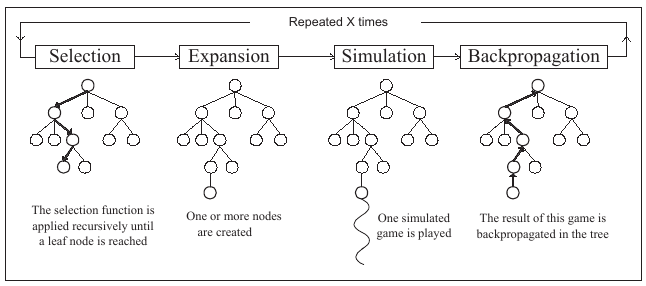
\includegraphics[width = 8.5cm]{Outline_MCTS}
    \caption{Outline of Monte Carlo Tree Search \cite{Chaslot2008}.}
    \label{fig:Outline_MCTS}
\end{figure}


This way, the algorithm uses a selection policy that balances exploration and exploitation to determine which nodes to expand next \cite{russell2020}. 
The first formula for balancing the two is called the Upper Confidence Bound 1 (UCB1). Upper Confidence Trees (UCT) is based on UCB1 formula and the Adaptive Multi-Stage Sampling algorithm \cite{Chang2005}, \cite{joppen2021}. The UCT formula used for this project is represented in Eq.~\ref{eq:UCT}.

% Eq.~\ref{eq:UCT}
\begin{equation}
    \label{eq:UCT}
    UCT = \frac{U(n)}{N(n)}\ + C \times \sqrt{\frac{2 \times ln(PARENT(n))}{N(n)}} 
\end{equation}

Where 
\begin{itemize}
    \item $U(n)$ is the total utility of node $n$
    \item $N(n)$ is the number of times node $n$ has been visited
    \item $PARENT(n)$ is the number of times the parent node of $n$ has been visited
    \item $C$ is a constant that determines the balance between exploration and exploitation
\end{itemize}

The utility $U(n)$ was applied as the difference between the number of wins and the number of loses of node $n$.

The constant $2$ inside the square root is used to scale the exploration term, such that it is proportional to the square root of the number of times the parent node has been visited. By scaling the exploration term with a constant inside the square root, the algorithm can adjust the degree of exploration based on the prior knowledge about the parent node \cite{joppen2021}.

The constant $C$ in the UCT formula (Eq.~\ref{eq:UCT}) defines the balance between exploration and exploitation. A higher value of $C$ will result in more exploration, while a lower value of $C$ will result in more exploitation. By choosing an appropriate value for $C$, the algorithm can balance the need for exploration with the need for exploitation, depending on the characteristics of the search space and the problem domain \cite{russell2020}.

In this work, a value of $2$ was chosen for constant $C$, determined by practical experimentation. It is worth noting that this value of $C$ results in a relatively high degree of exploration.
Lower values of $C$ have been shown to result in more exploitation and less exploration, which can be beneficial in some cases. However, in the practical experimentation conducted for this work, lower values of $C$ resulted in poorer results, indicating that a higher degree of exploration was needed to effectively search the search space.

Although MCTS can be applied in the absence of domain-specific knowledge, another significant aspect of MCTS is the use of this knowledge of the game rules, which can be used to bias the search towards positions that are more likely to lead to a win, achieving improvements in performance \cite{Browne2012}. 

In the specific case of this work, Eq.~\ref{eq:eval_func} was used to bias the search of the algorithm in the simulation phase. In each iteration of the simulation, the algorithm calculates all possible moves and applies Eq.~\ref{eq:eval_func} for scoring. After, the best scoring move is chosen as the next move of the rollout. The simplified pseudo-code can be found in Appendix~\ref{codeMC}.

It is worth mentioning, one possible way to improve the algorithm for future work would be to include the verification of the draw condition in this phase and use it to exclude that move or end the rollout early if that is the only possible move available. This can exceptionally decrease the decision-making process of the agent.

Regarding parameter setting for different board size and difficulties of the game, the maximum rollout depth (depth of simulation tree) and maximum number of iterations was adjusted. The values for these parameters can be found in Tab.~\ref{tab:MCTS_details}.

% Tab.~\ref{tab:MCTS_details}
\begin{table}[h]
    \caption{Parameter setting of different difficulty levels and board sizes for Monte Carlo Search Tree.}
    \centering
    \label{tab:MCTS_details}
        \begin{tabular}{l c c c c c c}
        \hline
        Difficulty & Board size & Rollout depth & Nº of iterations \\
        \hline
        Medium & 3x3 & 500 & 100\\
        Medium & 5x5 & $\infty$ & 100\\
        Medium & 9x5 & 500 & 10\\
        \addlinespace
        Hard & 3x3 & 500 & 200\\
        Hard & 5x5 & $\infty$ & 500 \\
        Hard & 9x5 & 500 & 20\\
        \hline
        \end{tabular}
\end{table}

% RESULTS AND DISCUSSION
\section{Results and Discussion}

As a result of this work, a python based program was developed that allows users to play Fanorona games in a variety of different configurations, with a user-friendly interface.

The computer performance was measured in different difficulties and board sizes, for all players (Random, Minimax, Minimax with Alpha-Beta pruning, and MCTS). Subsequently, the game results of 243 configurations were generated. The effectiveness of the algorithms was measured by their winning rate. It is interesting to mention that the human players failed to win any games against the AI agents. 

The game results of AI vs random players were evaluated, as well as the time duration, and the number of movements per game. The game time duration can be an important indication of the performance of the agents. For example, comparing the game time of MCTS vs. Minimax and MCTS vs. MCTS can allow an indirect indication of the speed of decision-making of the agents. The same argument applies to the total number of movements in a game.

The results showed that Minimax and Minimax with Alpha-Beta pruning algorithms win over Random player $100\%$ of the games, regardless of the difficulty and board size. Regarding the MCTS algorithm, it wins over random player $67\%$ of the games, as shown in Appendix~\ref{Appendix:resultsAIvsRandom}. The match between MCTS and the random player leads to a loss of MCTS or a draw in the bigger board sizes. This is due to the configurations of MCTS in bigger board sizes, which doesn't allow a deep enough search in the search tree and lacks a sufficient number of iterations to ensure a win, due to the big state space. This choice of configuration was taken in order to ensure the playability of the game within an acceptable time frame, as mentioned earlier.

Furthermore, each AI algorithm played against itself, in different difficulties (depths). This was done to evaluate the effectiveness of the AI in hard vs. medium mode. In all cases, the player with hard difficulty won over the player with medium difficulty. This confirms that the deeper the search tree, the more robust the agent becomes in the Fanorona game. 

According to Tab.~\ref{tab:AIvsRandom} in Appendix~\ref{Appendix:resultsAIvsRandom}, comparing the time per move for Minimax and Minimax with Alpha-Beta pruning in medium difficulty, we can confirm that Alpha-Beta pruning does indeed decrease the decision-making time for the agent. Regarding the hard difficulty, the comparison would not be valid, due to the different depths of the tree between the two agents (for details about the depths revisit Tab.~\ref{tab:Minimax_details}). 

Regarding the speed of decision-making of the agents, according to Tab.~\ref{tab:AIvsRandom} the average time per move of MCTS is higher in comparison to the other two agents, as the search space is much larger. This applies to all cases except for the medium difficulty on board size 9x5, which is understandable given that the number of iterations in this configuration is the smallest (Tab.~\ref{tab:MCTS_details}).

When MCTS agent played against all other AI agents, it was verified that even though in the smallest board size all agents are fast and have taken about the same amount of time to play against MCTS, in bigger board sizes MCTS is the slowest agent (Fig.~\ref{fig:mcts-time}). Moreover, we can conclude that MCTS playing against Minimax, Minimax with Alpha-Beta pruning, or random player, the game time durations are quite short and similar, making the three mentioned agents much faster than MCTS. This is understandable because the bigger the board gets, the bigger the search space, and the more time it takes for MCTS to explore the nodes. On the other hand, Minimax and Minimax with Alpha-Beta pruning players have a limited depth in the search tree and the time duration is not majorly impacted.

Next, all agents competed against the random agent to evaluate the number of movements per game (Fig.~\ref{fig:movespgame}). It was interesting to observe that in the smaller board size (3x3 and 5x5) MCTS is the agent that needs the least number of movements to finish the game. On the other hand, in the bigger board size, MCTS is the one that takes the most number of moves to finish the game. Again, this occurrence happens because of the configuration of the hyperparameters of MCTS agent in 9x5 board size, as mentioned before.

It is interesting to mention that in games of MCTS vs. Minimax or Minimax with Alpha-Beta pruning, the winners are consistent, as shown in Appendix~\ref{Appendix:resultsMinimaxvsMCTS} and Appendix~\ref{Appendix:resultsABvsMCTS}. This is expectable as the approaches of Minimax and Minimax with Alpha-Beta pruning are identical.

% Fig.~\ref{fig:mcts-time}
\begin{figure}[h!]
    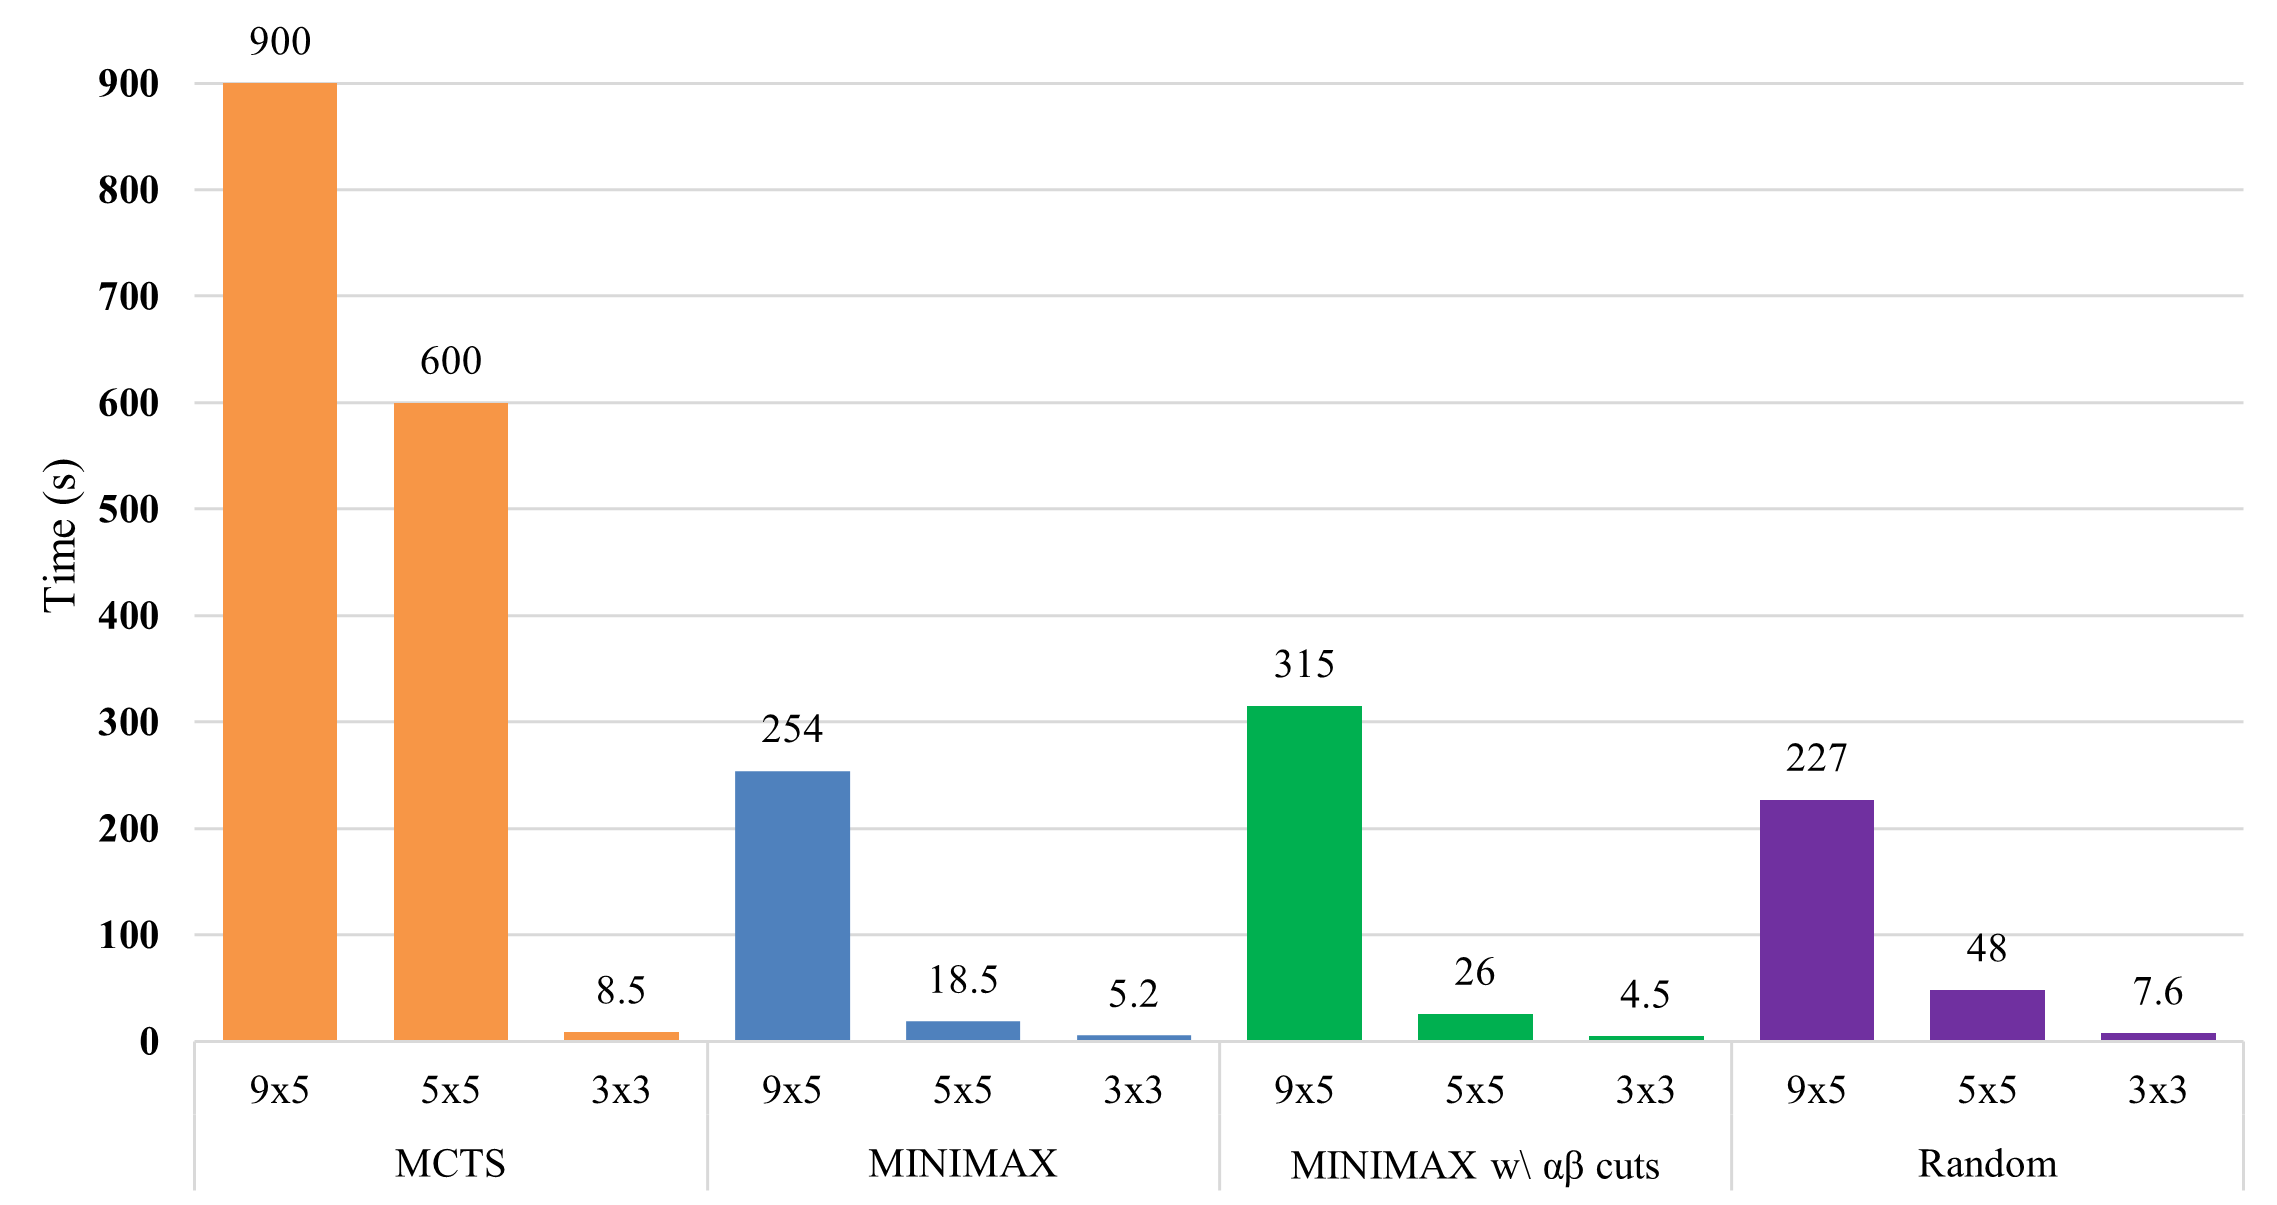
\includegraphics[width = 8.5cm]{mcts-time}
    \caption{MCTS agent games time duration.}
    \label{fig:mcts-time}
\end{figure}

% Fig.~\ref{fig:movespgame}
\begin{figure}[h!]
    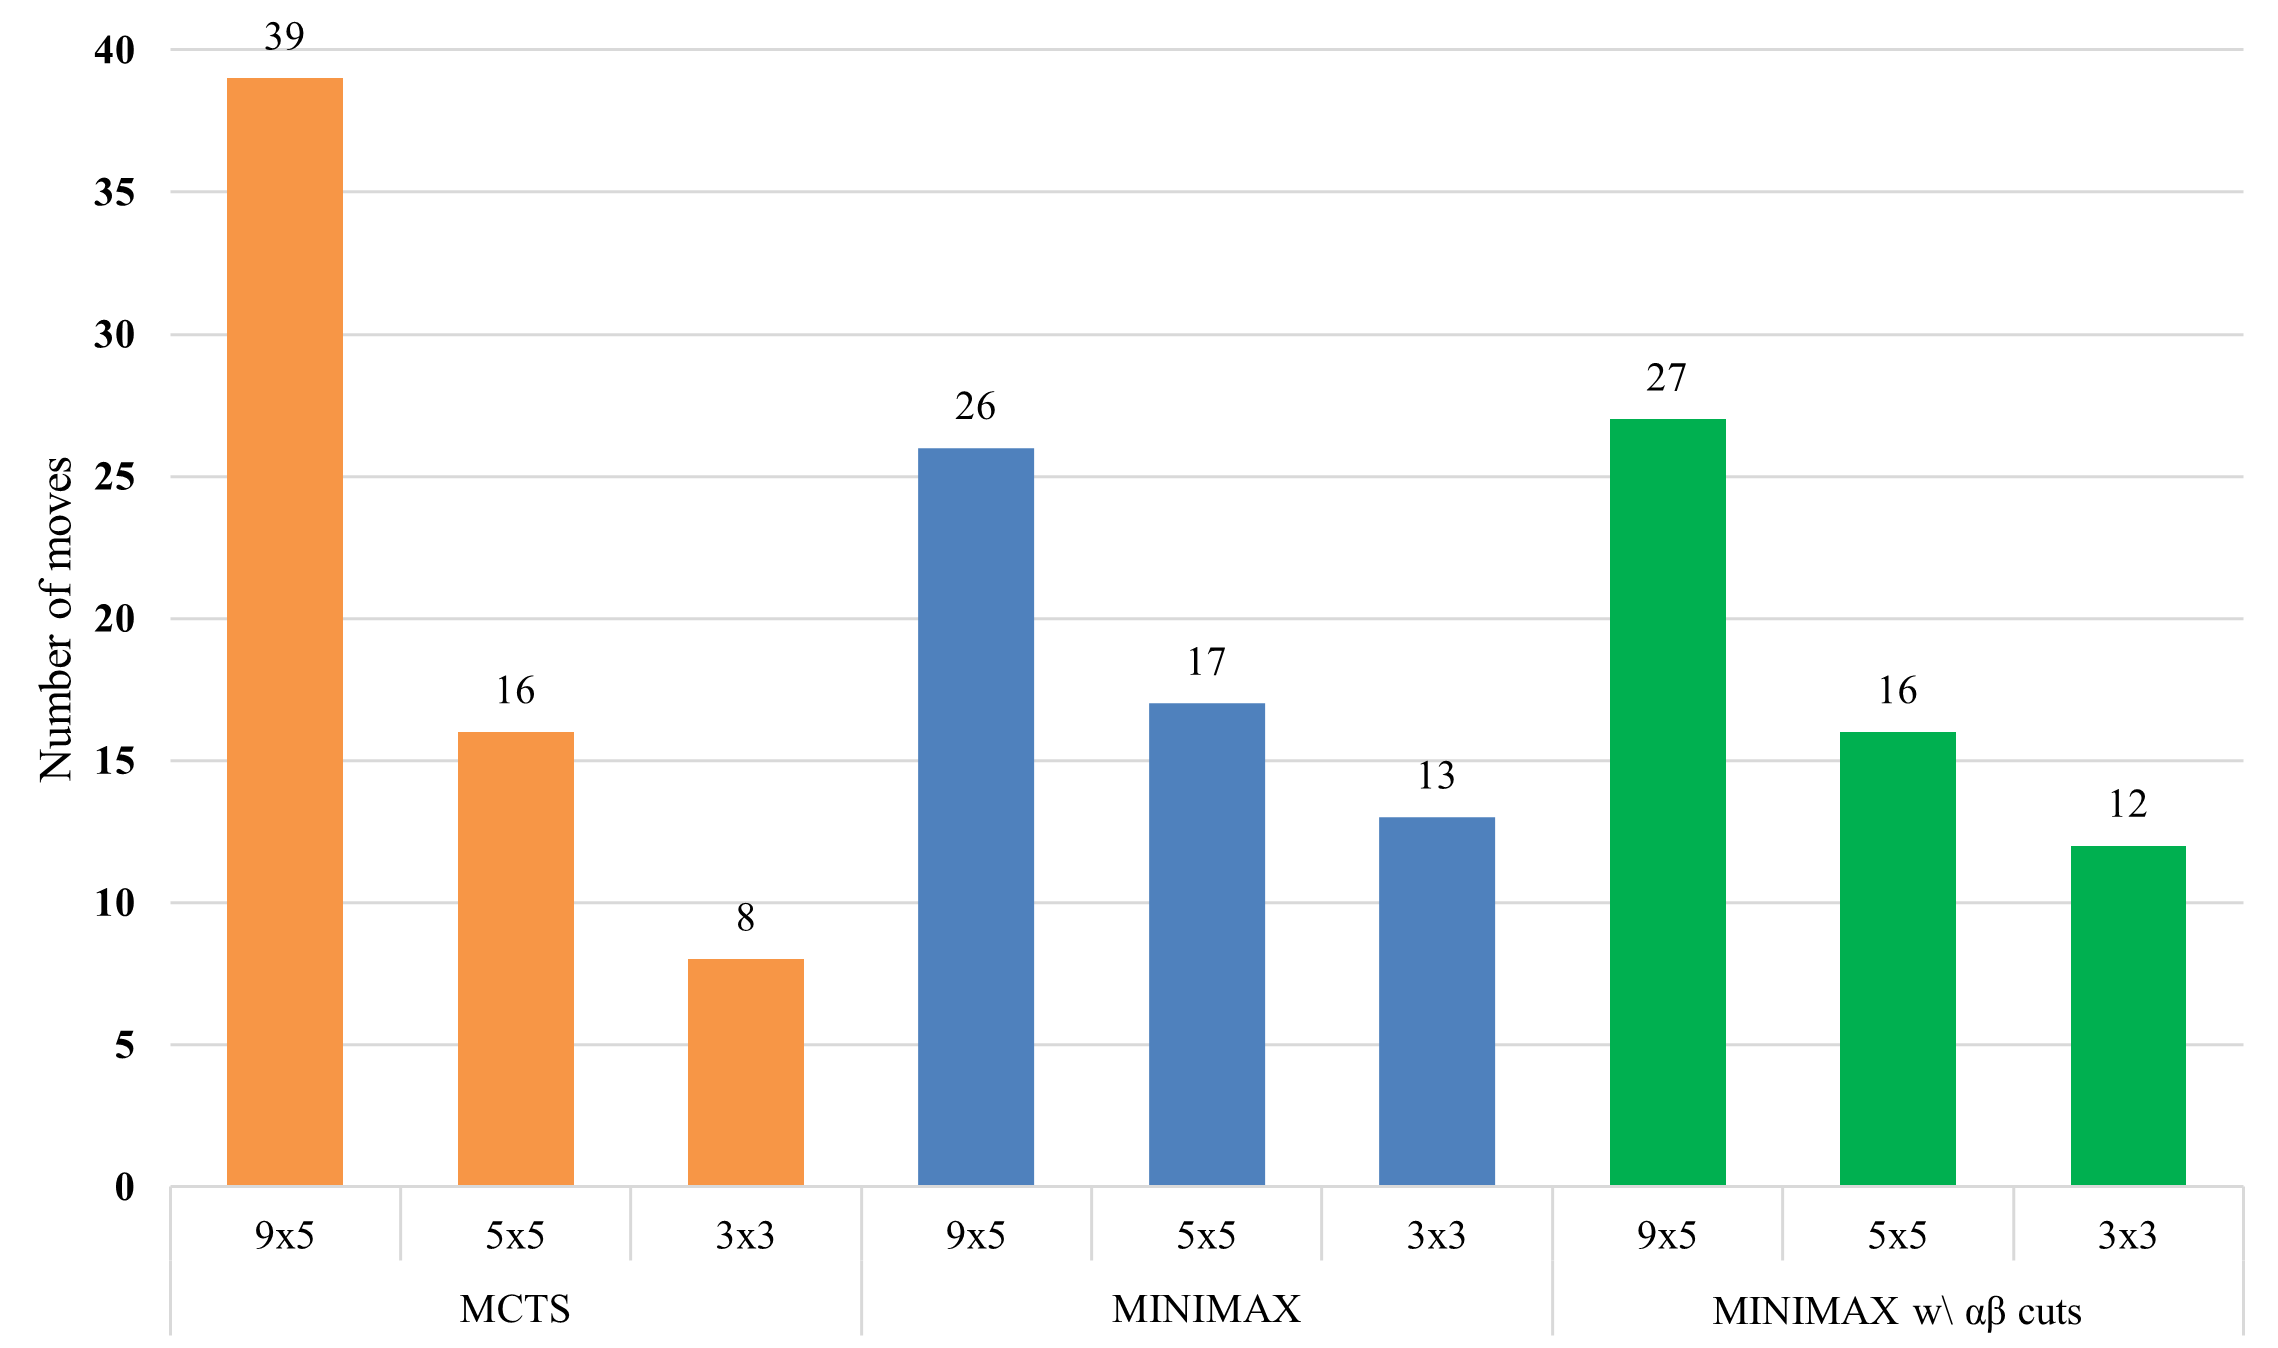
\includegraphics[width = 8.5cm]{movespgame}
    \caption{Number of moves per game - AI Agents against Random agent.}
    \label{fig:movespgame}
\end{figure}

\newpage
% CONCLUSIONS AND FUTURE WORKS
\section{Conclusion}

In this work, a Python-based Fanorona game was developed with various players, including a random player and 3 AI players - Minimax, Minimax with Alpha-Beta pruning, MCTS. 

Overall, it was confirmed that all AI players win against a random player. Minimax with Alpha-Beta pruning proves to be slightly faster than Minimax player. Both Minimax algorithms guarantee to find optimal moves regardless of the difficulty level and board size, but are computationally expensive and are prone to get stuck in loops. 

MCTS agent seems to be able to adopt a more offensive attitude, win the game in fewer moves, and play quite efficiently in smaller board sizes, but overall takes much longer to make a decision. In contrast with Minimax-based agents that in certain situations continuously avoid losing by entering a "loop" (Horizon problem, i.e., repeatedly deciding  to move between two places neither winning nor losing), MCTS more actively pursues strategies that in the long run lead to a win. For example, it was observed, MCTS was able to choose to lose one stone and in the next move was able to capture a number of opponents' stones that compensate for the initial loss. Altogether, both Minimax agents show promising results.

For future works, it would be interesting to allow the players to make consecutive moves in one turn. This option was not implemented in the current algorithm. It would also be interesting to explore other draw situations, especially for the AI players. 

Regarding the algorithm, in future works, it can definitely be optimized to decrease space complexity. 

Another interesting topic to explore further would be successor generation ordering in the Minimax algorithms. This can speed up the algorithm and reduce cases of draw, against other AI agents.

It would be important to future investigate the hyperparameter-tuning of the most relevant variables in UCB for MCTS. For MCTS the incorporation of draw condition in the rollout phase can possibly drastically decrease the computation time and improve its overall performance. 

\section*{Acknowledgment}
The authors would like to thank \emph{marcogx} and \emph{ahenrij} for sharing their codes for the Fanorona game on GitHub.

\vfill

\appendices
\section{Pseudo-Codes}
\label{code}
\subsection{Minimax}
\label{codeM}

    \begin{algorithm}[H]
    \caption{Minimax}\label{alg:cap1}
    \begin{algorithmic}
    
    \Function{play}{$game, state$}
        \State $player  \gets game.\Call{current\_player}{}$
      \State $ move  \gets \Call{Minimax-Search}{game, state}$
      \State $new\_state \gets game.\Call {Make-Move}{player, state, move}$
      \State \Return $new\_state$
    \EndFunction \\
    
    \Function{Minimax-Search}{$game, state$}
        \State $depth  \gets 0$
        \State $best\_v, best\_m \gets \Call{Max-Value}{game,  state, depth}  $
        \State \Return $best\_m$
    \EndFunction\\
    
    \Function{Max-Value}{$game, state, depth$}
        \If{$game.\Call{Is-Terminal}{state}$} 
        \State \Return $ game.\Call{Utility}{state, player}, null$
        \EndIf
        \State $value, move \gets -\infty$
        \ForAll{$m \in game.\Call{Get-Moves}{state, player}$}
        \State $n\_state \gets game.\Call{Make-Move}{player, state, m}$
          \State $v, m2 \gets \Call{Min-Value}{game, n\_state, depth+1}$
          \If{$v > value$}
            \State $value, move \gets v, m$
            
          \EndIf
        \EndFor
        \State \Return $value, move$
      \EndFunction\\
    
    \Function{Min-Value}{$game, state, depth$}
      \If{$depth \geq game.$difficulty} 
      \State  \Return $game.\Call{Utility}{state, player}, null$
      \EndIf
      \If{$game.\Call{Is-Terminal}{state}$} 
        \State \Return $ game.\Call{Utility}{state, player}, null$
        \EndIf
        \State $value, move \gets +\infty$
        \ForAll{$m \in game.\Call{Get-Moves}{state, player}$}
        \State $n\_state \gets game.\Call{Make-Move}{player, state, m}$
          \State $v, m2 \gets \Call{Max-Value}{game, n\_state, depth+1}$
          \If{$v < value$}
            \State $value, move \gets v, m$
            
          \EndIf
        \EndFor
        \State \Return $value, move$
      \EndFunction
    
    
    \end{algorithmic}
    \end{algorithm}

\newpage
% Appendix~\ref{Appendix:codeAB}
\subsection{Minimax with Alpha-Beta cuts}
\label{Appendix:codeAB}

\begin{algorithm}[H]
\caption{Minimax with Alpha-Beta cuts}\label{alg:cap2}
\begin{algorithmic}
\Function{play}{$game, state$}
    \State $player  \gets game.\Call{current\_player}{}$ 
  \State $ move  \gets \Call{Minimax-AlphaBeta-Search}{game, state}$
  \State $new\_state \gets game.\Call {Make-Move}{player, state, move}$
  \State \Return $new\_state$
\EndFunction \\

\Function{Minimax-AlphaBeta-Search}{$game, state$}
    \State $depth  \gets 0$
    \State $best\_v, best\_m  \gets \Call{Max-Value}{game, state, \par\hfill depth, -\infty, +\infty}$
    \State \Return $best\_m$
\EndFunction\\

\Function{Max-Value}{$game, state, depth, \alpha, \beta$}
    \If{$game.\Call{Is-Terminal}{state}$} 
    \State \Return $ game.\Call{Utility}{state, player}, null$
    \EndIf
    \State $value, move \gets -\infty$
    \ForAll{$m \in game.\Call{Get-Moves}{state, player}$}
    \State $n\_state \gets game.\Call{Make-Move}{player, state, m}$
      \State $v, m2 \gets \Call{Min-Value}{game, n\_state, depth+1}$
      \State $\alpha \gets \Call{Max}{\alpha, v} $
      \If{$v \geq \beta$}
        \State \Return $value, move \gets v, m$
        
      \EndIf
    \EndFor
    \State \Return $value, move$
  \EndFunction\\

\Function{Min-Value}{$game, state, depth, \alpha, \beta$}
  \If{$depth \geq game.$difficulty} 
  \State  \Return $game.\Call{Utility}{state, player}, null$
  \EndIf
  \If{$game.\Call{Is-Terminal}{state}$} 
    \State \Return $ game.\Call{Utility}{state, player}, null$
    \EndIf
    \State $value, move \gets +\infty$
    \ForAll{$m \in game.\Call{Get-Moves}{state, player}$}
    \State $n\_state \gets game.\Call{Make-Move}{player, state, m}$
      \State $v, m2 \gets \Call{Max-Value}{game, n\_state, depth+1}$
      \State $ \beta  \gets \Call{Min}{\beta, v}$
      \If{$v \leq \alpha$}
        \State \Return $value, move \gets v, m$
        
      \EndIf
    \EndFor
    \State \Return $value, move$
  \EndFunction


\end{algorithmic}
\end{algorithm}

\newpage
\subsection{Monte Carlo Tree Search}
\label{codeMC}

\begin{algorithm}[H]
\caption{Monte Carlo Tree Search (simplified)}\label{alg:cap3}
\begin{algorithmic}
\Function{play}{$game, state$}
    \State $player  \gets game.\Call{current\_player}{}$ 
  \State $ move  \gets \Call{MonteCarlo-Search}{game, state,$ \par\hfill $max\_rollout\_depth, n\_iterations, 2$}
  \State $new\_state \gets game.\Call {Make-Move}{player,$ \par\hfill $state, move$}
  \State \Return $new\_state$
\EndFunction \\


\Function{MonteCarlo-Search}{$game, state,$  \par\hfill $  max\_rollout\_depth, n\_iterations, C$}

    \State $root  \gets \Call{Node}{game, state}$
    \For {$ i \in [0, n\_iterations[$}
    \State $\Call{Run-Iteration}{game, state,$ \par\hfill $max\_rollout\_depth, C$}
    \EndFor
    \State $best\_child \gets root.\Call{best\_child}{C}$
    \State $move, node \gets best\_child.\Call{Parent}{} $
    \State \Return $move$
\EndFunction\\

\Function{Run-Iteration}{$game, state,$ \par\hfill $max\_rollout\_depth, C$}
    \State $current\_n \gets root$
    \While{\textbf{not} $ game.\Call{Is-Terminal}{current\_n.state}$}{
    \State $current\_n.\Call{Expand}{}$
    \State $current\_n.\Call{Simulate}{}$
    \State $current\_n \gets  current\_n.\Call{best\_child}{C}$
    }
    \State $current\_n.\Call{Back-propagate}{}$
  \EndFunction
\end{algorithmic}
\end{algorithm}


% Appendix~\ref{Appendix:resultsMinimaxvsAB}
\section{Minimax vs. Minimax with Alpha-Beta pruning}
\label{Appendix:resultsMinimaxvsAB}
% Tab.~\ref{tab:MinimaxvsAB}
\begin{table}[h!]
    \caption{Game results of Minimax agent vs. Minimax with Alpha-Beta pruning agent in different difficulty levels and board sizes. Difficulty level indicates the difficulty level applied for both agents, according to the details mentioned in Section~\ref{section:Methodology}. Results were generated running on an Intel(R) Core(TM) i7-8750H CPU @ 2.20GHz and 16.0GB RAM computer.}
    \centering
    \label{tab:MinimaxvsAB}
        \begin{tabular}{l c c c c}
        \hline
        Difficulty & Size & Winner & Time (s) & Moves \\
        \hline
        Medium & 3x3 & Minimax               & 0.8 & 13 \\
        Medium & 5x5 & Minimax-$\alpha\beta$ & 1.7 & 26 \\
        Medium & 9x5 & Minimax               & 1.8 & 43 \\
        \addlinespace
        Hard   & 3x3 & Minimax               & 0.6 & 10 \\
        Hard   & 5x5 & Draw                  & 4.1 & 33 \\
        Hard   & 9x5 & Minimax-$\alpha\beta$ & 91.9 & 30 \\
        \hline
        \end{tabular}
\end{table}

\newpage
% Appendix~\ref{Appendix:resultsMinimaxvsMCTS}
\section{Minimax vs. MCTS}
\label{Appendix:resultsMinimaxvsMCTS}
% Tab.~\ref{tab:MinimaxvsMCTS}
\begin{table}[h!]
    \caption{Game results of Minimax agent vs. MCTS agent in different difficulty levels and board sizes. Difficulty level indicates the difficulty level applied for both agents, according to the details mentioned in Section~\ref{section:Methodology}. Results were generated running on an Intel(R) Core(TM) i7-8750H CPU @ 2.20GHz and 16.0GB RAM computer.}
    \centering
    \label{tab:MinimaxvsMCTS}
        \begin{tabular}{l c c c c}
        \hline
        Difficulty & Size & Winner & Time (s) & Moves\\
        \hline
        Medium & 3x3 & MCTS & 10.1 & 13\\
        Medium & 5x5 & Minimax & 8.7 & 17\\
        Medium & 9x5 & MCTS & 140.1 & 25\\
        \addlinespace
        Hard & 3x3 & MCTS & 6.6 & 10 \\
        Hard & 5x5 & MCTS & 46.5 & 22\\
        Hard & 9x5 & Minimax & 429.6 & 35\\
        \hline
        \end{tabular}
\end{table}

 
% Appendix~\ref{Appendix:resultsAIvsRandom}
\section{AI vs Random}
\label{Appendix:resultsAIvsRandom}
% Tab.~\ref{tab:AIvsRandom}
\begin{table}[h!]
    \caption{Game results of Random agent vs. different AI agents in different difficulty levels and board sizes. Size refers to the board size. "t" represents the time of the whole game, and t/M represents the average time per move for the players in the game. Results were generated running on a Intel(R) Core(TM) i7-8750H CPU @ 2.20GHz and 16.0GB RAM computer.}
    \centering
    \label{tab:AIvsRandom}
        \begin{tabular}{c l c c c c c}
        \hline
        AI & Difficulty &  Size & Winner & t (s) & Moves & $\overline{t/M (s)}$ \\
        \hline
        \multirow{6}{*}{\rotatebox[origin=c]{90}{Minimax}}
         & Medium & 3x3 & AI & 0.9 & 13 & 0.07\\
         & Medium & 5x5 & AI & 1.0 & 16 & 0.06\\
         & Medium & 9x5 & AI & 2.5 & 26 & 0.10\\
         & Hard & 3x3 & AI & 0.7 & 12 & 0.06\\
         & Hard & 5x5 & AI & 2.8 & 18 & 0.16\\
         & Hard & 9x5 & AI & 2.5 & 26 & 0.10\\
        \addlinespace  
        \multirow{6}{*}{\rotatebox[origin=c]{90}{Minimax-$\alpha\beta$}}
         & Medium & 3x3 & AI & 0.9 & 14 & 0.06\\
         & Medium & 5x5 & AI & 1.0 & 16 & 0.06\\
         & Medium & 9x5 & AI & 1.6 & 24 & 0.07\\
         & Hard & 3x3 & AI & 0.7 & 12 & 0.06\\
         & Hard & 5x5 & AI & 1.5 & 18 & 0.08\\
         & Hard & 9x5 & AI & 6.8 & 30 & 0.23\\
        \addlinespace
        \multirow{6}{*}{\rotatebox[origin=c]{90}{MCTS}}
         & Medium & 3x3 & AI & 4.2 & 10 & 0.42 \\
         & Medium & 5x5 & Draw & 7.3 & 16 & 2.19 \\
         & Medium & 9x5 & AI & 1.2 & 36 & 0.03 \\
         & Hard & 3x3 & AI & 6.6 & 10 & 0.66 \\
         & Hard & 5x5 & AI & 37.8 & 23 & 1.64 \\
         & Hard & 9x5 & Random & 48.0 & 39 & 1.23\\
        \hline
        \end{tabular}
\end{table}

\newpage
% Appendix~\ref{Appendix:resultsABvsMCTS}
\section{MCTS vs. Minimax with Alpha-Beta pruning}
\label{Appendix:resultsABvsMCTS}
% Tab.~\ref{tab:ABvsMCTS}
\begin{table}[h!]
    \caption{Game results of MCTS agent vs. Minimax with Alpha-Beta pruning agent in different difficulty levels and board sizes. Difficulty level indicates the difficulty level applied for both agents, according to the details mentioned in Section~\ref{section:Methodology}. Results were generated running on an Intel(R) Core(TM) i7-8750H CPU @ 2.20GHz and 16.0GB RAM computer.}
    \centering
    \label{tab:ABvsMCTS}
        \begin{tabular}{l c c c c}
        \hline
        Difficulty & Size & Winner & Time (s) & Moves \\
        \hline
        Medium & 3x3 & MCTS                  &  0.8 & 13 \\
        Medium & 5x5 & Minimax-$\alpha\beta$ & 14.8 & 24 \\
        Medium & 9x5 & MCTS                  & 414.1 & 57 \\ 
        \addlinespace
        Hard & 3x3 & MCTS                   & 9.2 & 10 \\
        Hard & 5x5 & MCTS                   & 68.2 & 22 \\
        Hard & 9x5 & Minimax-$\alpha\beta$  & 1279.7 & 37 \\
        \hline
        \end{tabular}
\end{table}

\ifCLASSOPTIONcaptionsoff
  \newpage
\fi

% Bibliography
\small
\bibliographystyle{ieeetr}
\addcontentsline{toc}{chapter}{References}
\bibliography{report.bib} % includes the file ./refs/report.bib
\normalsize

\end{document}

